\section{Pseudonymisierung}

\label{sec_basics_pseudonymity}

Ein Pseudonym\footnote{
	ursprünglich aus dem Griechischen stammend: \textit{pseudonumon} - falsch benannt
} bezeichnet nach \cite{pfitzmann2010} einen Identifikator eines Subjekts ungleich seinem echten Bezeichner. In §3, Absatz (6a) des BDSG wird zusätzlich noch der \glqq Zweck [eines Pseudonyms], die Bestimmung des Betroffenen auszuschließen oder wesentlich zu erschweren\grqq{}\cite{TODO} ergänzt. Beispiele für Pseudonyme lassen sich in verschiedensten Bereichen finden: E-Mail-Adressen, Sozialversicherungsnummern oder auch Autoren, die unter einem Pseudonym ihre Schriften veröffentlichen.\todo{Evtl. auch Telemediengesetz erwähnen - Nutzung eines Systems unter einem Pseudonym}

Es lassen sich nach \cite{pfitzmann1990} unterschiedliche Arten von Pseudonymen unterscheiden. Eine Eigenschaft, die zur Unterscheidung herangezogen werden kann, ist die (Un-)Kenntnis des Zusammenhangs zwischen dem Pseudonym und dem zugehörigen Subjekt zu Beginn seiner Verwendung. Dieser Zusammenhang wird auch als Zuordnungsvorschrift bezeichnet und kann beispielsweise als Funktion oder in Tabellenform vorliegen.s\\
Hier kann zwischen öffentlichen, nicht-öffentlichen und anonymen Pseudonymen unterschieden werden. Ein öffentliches Pseudonym ist beispielsweise die Telefonnummer einer Person, die von Beginn an im Telefonbuch mit der Identität der Person verknüpft ist. Eine Kontonummer zu einem Bankkonto, dessen Inhaber bei der Kontoeröffnung nur der Bank bekannt ist, bildet ein nicht-öffentliches Pseudonym. Ein anonymes Pseudonym bildet beispielsweise die DNA-Sequenz eines Menschen, die oftmals nicht einmal ihm selbst bekannt ist. Diese Eigenschaft eines Pseudonyms kann sich im Laufe der Zeit ändern, wenn Informationen über den Zusammenhang zwischen Pseudonym und zugehörigem Subjekt veröffentlicht werden.

Eng in Verbindung mit Pseudonymen steht auch der Begriffe der Verkettbarkeit. 
Verkettbarkeit bezeichnet dabei die Eigenschaft, dass ein Außenstehender mit hoher Wahrscheinlichkeit entscheiden kann, ob zwei Objekte in einem System unabhängig sind\cite{pfitzmann2010}.

Auf Basis dieser Eigenschaft lassen sich nun ebenfalls verschiedene Arten von Pseudonymen ausmachen:
Diese Arten unterscheiden sich durch Nutzung des Pseudonyms in verschiedenen Kontexten. Personen-, Rollen-, Beziehungs-, Rollen-Beziehungs- und Transaktionspseudonym sind mögliche Ausprägungen dieser Eigenschaft. Eine Übersicht über diese Pseudonymarten und deren Zusammenhang zur Verkettbarkeit ist Abbildung \ref{fig:lattice_pseudonym} zu entnehmen.\\
Personenpseudonyme beschreiben Pseudonyme wie beispielsweise die Sozialversicherungsnummer, die stellvertretend für die eindeutige Identität des Subjekts in der Gesellschaft stehen. Ereignisse, die mit solchen Pseudonymen verbunden sind, lassen sich über die gesamte Gültigkeitsspanne des Pseudonyms verketten. \\
Rollen-, Beziehungs- und Rollen-Beziehungspseudonyme stellen Pseudonyme da, die das Subjekt nur in einer besonderen Funktion oder mit einem bestimmten Kommunikationspartner bzw. in der Kombination beider Möglichkeiten nutzt. Ein Beispiel hierfür wäre eine E-Mail-Adresse wie \textit{administrator@unternehmen.de} in einem Unternehmen, die nicht das Subjekt als solches sondern nur in seiner Rolle in dem Unternehmen beschreibt. Ereignisse verknüpft mit diesen Pseudonymarten lassen sich nur in bestimmten Kontexten, jedoch nicht über diese hinweg, verknüpfen. Beispielsweise könnten zwei Kommunikationspartner mit derselben Person kommunizieren ohne dies feststellen zu können, wenn die Person unter unterschiedlichen Beziehungspseudonymen auftritt.\\
Transaktionspseudonyme stellen die stärkste Form der Unverkettbarkeit da. Bei dieser Art von Pseudonymen wird für jedes Ereignis ein neues Pseudonym verwendet, das daher nur ein einziges Mal auftritt und Verkettbarkeit verhindert.\\

\begin{figure}[]
    \centering
        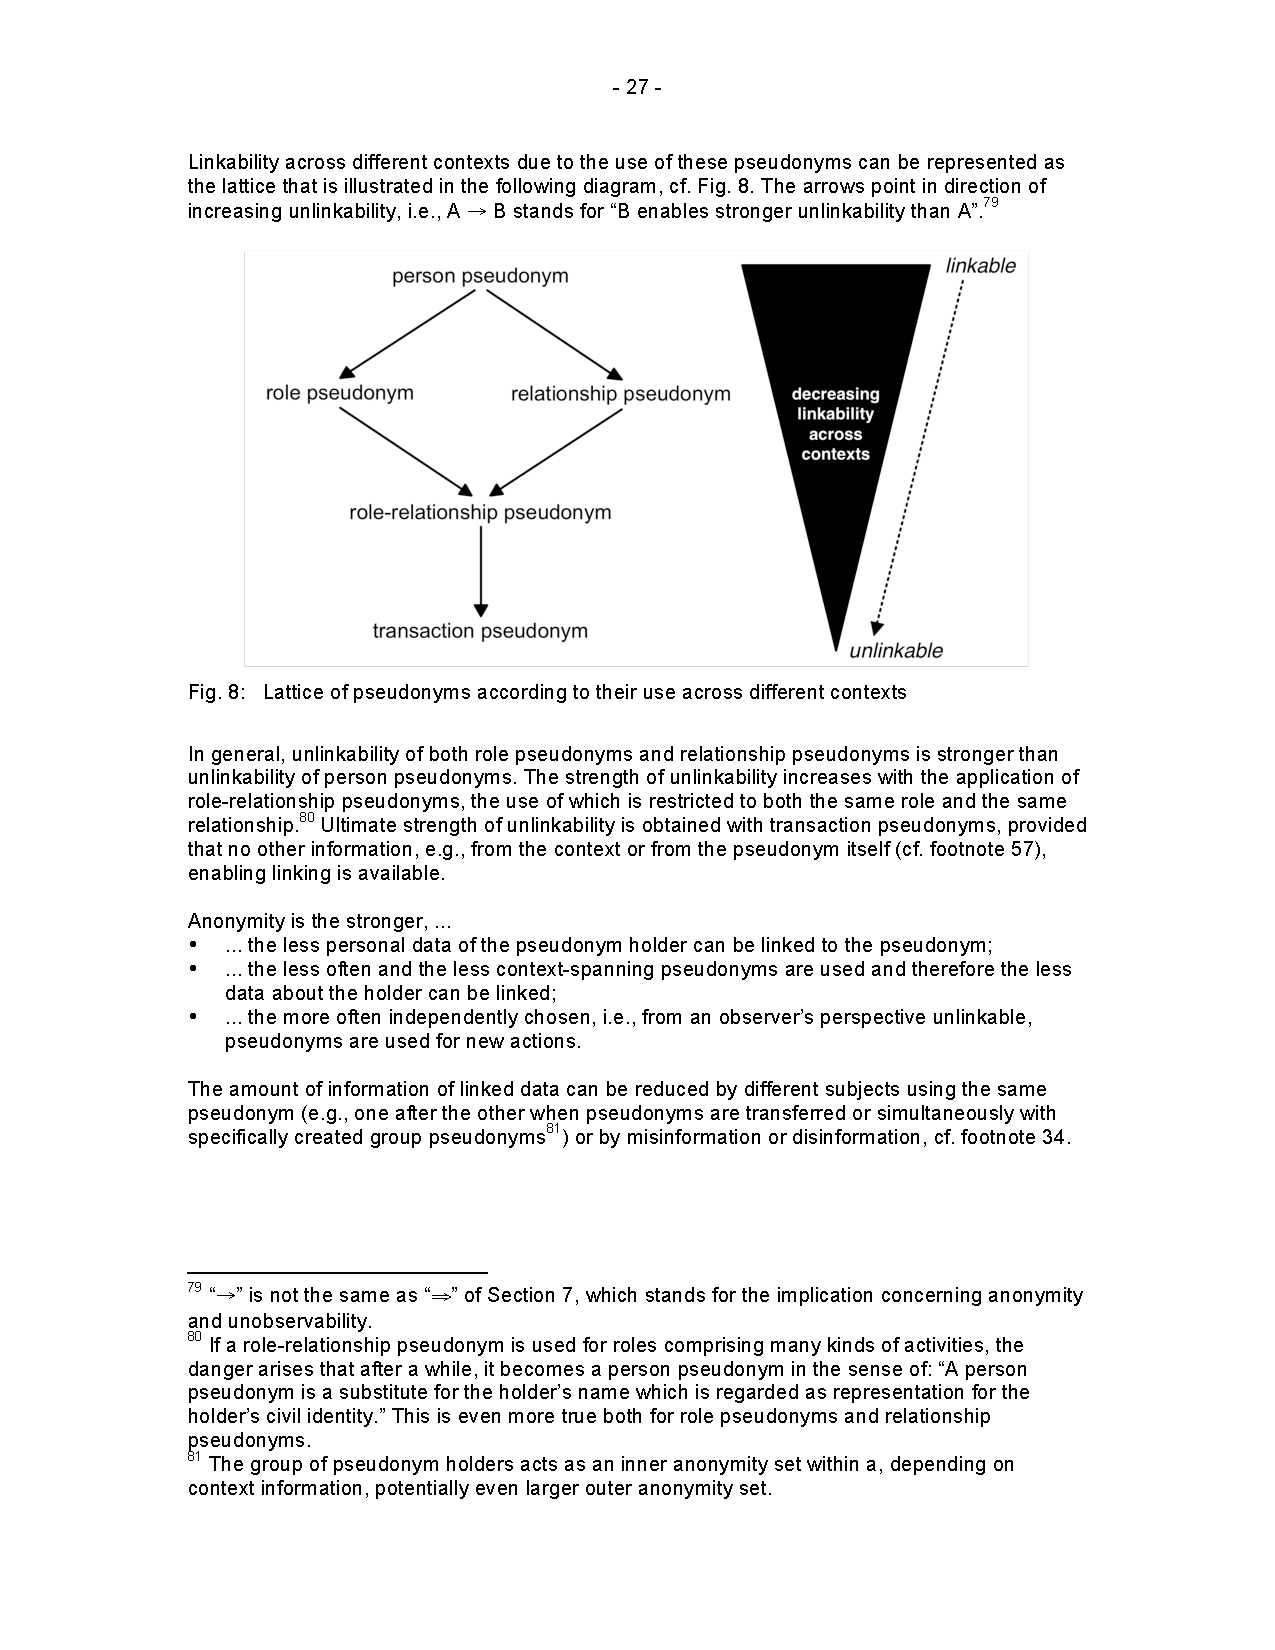
\includegraphics[clip, trim=0cm 16.5cm 0cm 4cm, width=1.00\textwidth]{img/pseudonym_lattice_excerpt.pdf}
    \caption{Pseudonym-Verband entsprechend ihrer Nutzung in verschiedenen Kontexten. Entnommen aus \cite{pfitzmann2010}.}
    \label{fig:lattice_pseudonym}
\end{figure}

\tbc{Abgrenzung zur Anonymität sinnvoll?}

\tbc{Ist der \glqq Schnitt\grqq{} zwischen Kapitel 2 und 3 hier sinnvoll?}